\chapter{Work performed}
\setlength{\parskip}{2.5ex plus .4ex minus .4ex}
\section{Controller}\label{sec:controller}
Each ``Controller'' associated to an agent on the world inherit from the main class ``Controller'' of SIGVerse. That is why each of them has the same dynamic shown figure~\ref{fig:controllerDyn}.\\

When the simulation starts on the SIGViewer, each ``Controller'' is initialized running ``onInit'' method. After that the ``onAction'' method is running regularly, it can be every 1 seconds like 0.1, 0.5,... It is defined by the return value of ``onAction'' method.\\
If a collision occurs between the agent and something else, ``onCollision'' is executed.\\
If the agent receives a message, ``onRecvMsg'' is executed.\\

In any case, ``onAction'' is running until the simulation stops. If the simulation restarts, ``onInit'' is not executed, the simulation continues where it stopped.\\

\noindent\begin{minipage}{\linewidth}% to keep image and caption on one page
\makebox[\linewidth]{%        to center the image
  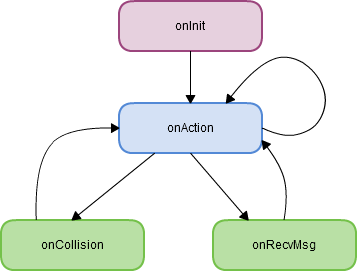
\includegraphics [width=100mm]{images/controllerDyn.png}}
\captionof{figure}{Dynamic of the ``Controller''}\label{fig:controllerDyn}%      only if needed  
\end{minipage}

\section{Architecture}
\subsection{General objective}
On the SIGServer, severals ``Controller'' can run at the same time, because there are one for each agent in the simulator and their types can be different. For exemple, we can have a ``Controller'' for a Robot and ``Controller'' for an object. The principal difference between them is that a Robot controller do not apply the same method to the agent than an object, indeed the robot can move, not an object. But they have the same dynamic, section~\ref{sec:controller}.\\
If we have three robots in the simulator, that means three ``Controller''.\\

We can see figure~\ref{fig:sig_ros_general} how the interface has to work. Several nodes can send information to topics which can be the same or not. This is the ROS part. And these topics are subscribed by the ``Controller'' of SIGServer.\\
As we can see, the same node can publish to the same node ``Topic 4'' or one node can publish to several nodes ``Node 1''.\\
However, different ``Controller'' cannot publish or subscribe to the same topic. The reason is that the ROS user do not have to write the ``Controller'' or edit it neither, it will be generated and I can not know if the user want the same behaviour between two or more agents. If the user wants this behaviour, he will have to send the same message to severals topics.\\

As we can see figure~\ref{fig:sig_ros_general} a service can be called too. The difference with publishing/subscribing is that a request is sent and the ``Controller'' will answer with a response to the node who asked ``Node 3''.

\noindent\begin{minipage}{\linewidth}% to keep image and caption on one page
\makebox[\linewidth]{%        to center the image
  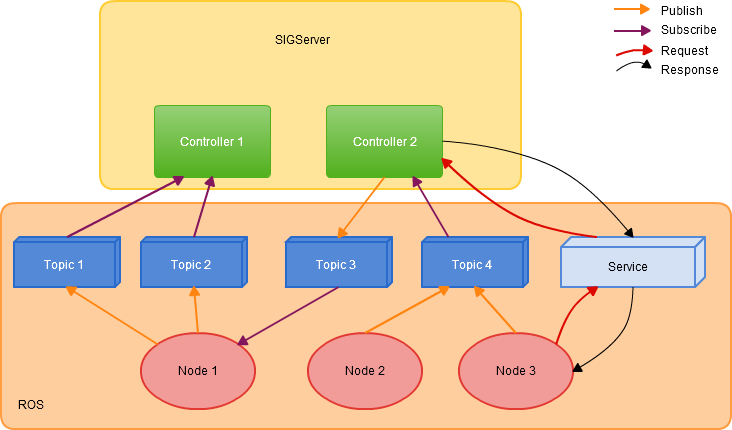
\includegraphics [width=150mm]{images/sig_ros_general.png}}
\captionof{figure}{Many ROS nodes send and receive information to many controllers}\label{fig:sig_ros_general}%      only if needed  
\end{minipage}

\subsection{Controllers used}
As explained earlier, one ``Controller'' is associated to one agent for making him act. This association is defined in the xml file which describes the agent.\\
The same ``Controller'' can be associated to several agents, that means that all agent associated to this ``Controller'' will act the same.\\
On this project, ``Controllers'' has to be developped for creating topics which sent information and make the agent acting. So, two ``Controllers'' will be necessary, one for the robot and one for the object. For generals methods like getting entities, they can be included on the object controller.\\
The best would be a general controller for the methods in common to avoid the duplication of topics, but for this mid-term report, only the robot controller and the object controller are implemented with the methods inside them.\\
So, in our case, I have as many topics (or services) for getting entities as number of agent in the simulator.\\

The robot ``Controller'' inherits from the object ``Controller'' called ``SimObjController''. The reason is that in SIGVerse, a robot is an object and has only two methods more than on the object ``Controller''.\\

\subsection{Package}
ROS is an open source framework who works with packages, every extension is a package. So, the ROS users just need to download the package wanted.\\
That is why I choose to develop a package, and only running the node called ``ros\_controller'' will be necessary to launch the SIGServer, create the ``Controllers'', the topics and services.\\
We can see figure~\ref{fig:sig_ros_package} the composition of the package.
\begin{description}
	\item[src] : The generic ``Controller'' for each kind of agent.
	\item[srv] : The definition of each services needed.
	\item[msg] : The definition of each messages needed.
	\item[tests] : Tests files to check the validity of the implementation.
\end{description}

\noindent\begin{minipage}{\linewidth}% to keep image and caption on one page
\makebox[\linewidth]{%        to center the image
  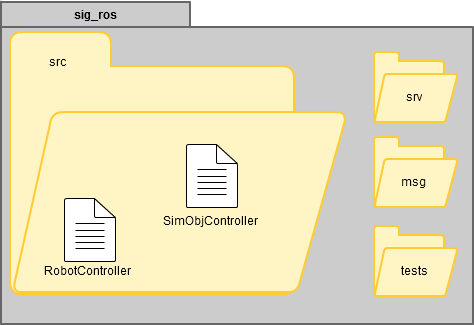
\includegraphics [width=120mm]{images/package_sig_ros.png}}
\captionof{figure}{sig\_ros package}\label{fig:sig_ros_package}%      only if needed  
\end{minipage}

\section{Usage}
From the user point of view, three steps are important, see figure~\ref{fig:usage}.\\
First, the user launches the sig\_ros package. So, the SIGServer is automatically launched and the SIGViewer can be connected.\\
Second, the user starts the simulation from the SIGViewer. So, all topics and services are created and linked to the ``Controller'' thanks to the package sig\_ros.\\
Finally, the user can create all the ROS node he wants and publish and subscribe to the topics and call services created by the step 2.

\noindent\begin{minipage}{\linewidth}% to keep image and caption on one page
\makebox[\linewidth]{%        to center the image
  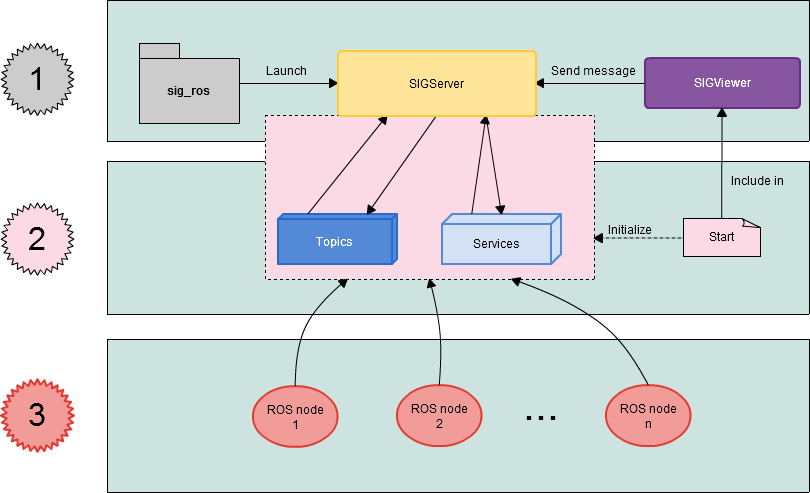
\includegraphics [width=150mm]{images/usage.png}}
\captionof{figure}{Steps to follow to start a simulation with ROS}\label{fig:usage}%      only if needed  
\end{minipage}

\section{Topics \& Services}
\subsection{Generalities}
Topics and services have to be defined. A node which subscribe to a topic receive the message as soon as it is published to the topic but no answer is given.\\
On the contrary, the service is a topic but it anwsers to the node who called the service.\\
The types of messages or service request can be of several simple type (double, string, ...) or a combination of these type or message created by these types.\\
It is possible to create new types, so the tranfert of SIGVerse object could be possible, but the use of the package has to be as easy as possible. So, the methods needed by the clean up task which return bad type for a message are replaced by a topic or service which execute a group of action, for exemple getPart and getPosition applied to the part are mixed in getPartPosition and the user only has to ask for a part and the position is returned with simple type ``double''.\\

The first step is to make the example of the clean up task working, so many topics and services have been created. Each of them starts by the name of the agent and follow by the name of the topic/service.

Now, we are going to see the topics and services I implemented for the robot agent, but a more exhaustive list with more details is given in annex~\ref{annex:topics} and annex~\ref{annex:services}. In those annexes, there are the topics for the robot agent but also for the object agent of the clean up task which I have started implementing.

\subsection{Topics}
The list of the topics needed for the robot agent of the clean up task is:
\begin{description}
	\item[\_onRecvMsg] : The ``Controller'' send the message received by the SIGViewer.
	\item[\_onCollisionMsg] : The name of the agent which one is in collision with are sent to this topic. If there is severals collision at the same time, severals messages are sent.
	\item[\_setWheel] : Publish the radius and the distance in a message and they will be applied to the robot.
	\item[\_setWheelVelocity] : Publish the velocity for the left and the right wheel and it will be applied.
	\item[\_setJointVelocity] : set the velocity ``angular velocity'' to the join called ``jointName''.
	\item[\_releaseObj]: Publish the part which you want to release an object and it will be done.
\end{description}

The two first topics was obvious, they are the unique topics where the ``Controller'' publish. Indeed, the dynamic of the ``Controller'' run two methods when particular events occurs, see section~\ref{sec:controller}. That is why, each time it occurs, messages are sent to this topics.

\subsection{Services}
The list of the services needed for the robot agent of the clean up task is:
\begin{description}
	\item[\_get\_time] : Get the simulation time.
	\item[\_get\_obj\_position] : Get the position of the object named name, if name is empty, return the position of the agent which the service's name start with.
	\item[\_get\_parts\_position] : Get the position of the part in parameter.
	\item[\_get\_rotation] : Get the quaternion of the agent's rotation.
	\item[\_get\_angle\_rotation] : Get the angle of the rotation of the agent.
	\item[\_get\_joint\_angle]: Get the angle between the joint.
	\item[\_grasp\_obj]: Grasp the object ``obj'' with the part ``part''.
\end{description}


\section{SIGViewer service}
SIGViewer give a graphic interface for the visualization of the world and the robot. But many services can be connected to SIGViewer for example the referee of the Robocup competition.\\
The connection with the service is made at the SIGViewer level as we can see figure~\ref{fig:referee}. The user only has to install the service and add it to the SIGViewer. After that, the interaction with the service from the SIGServer is possible. Indeed, SIGServer is connected to the SIGViewer and the SIGViewer with the service.\\
Server side, the controller just need to send a message to the SIGViewer to connect with the service. After that, the controller can send every messages wanted to the service.\\

\noindent\begin{minipage}{\linewidth}% to keep image and caption on one page
\makebox[\linewidth]{%        to center the image
  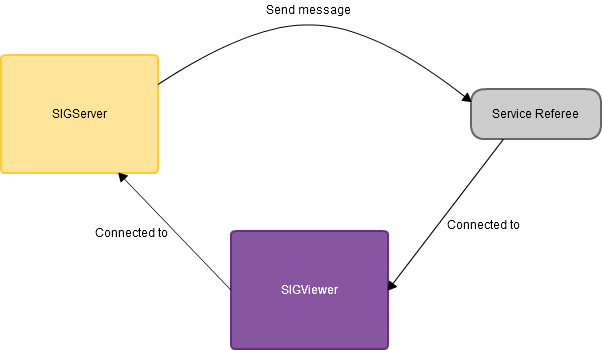
\includegraphics [width=150mm]{images/referee.png}}
\captionof{figure}{Links between SIGServer, SIGViewer and the referee service}\label{fig:referee}%      only if needed  
\end{minipage}

Basically, only few methods are related to the SIGViewer service, one for the connection, another for checking the connection and a last one for sending messages to the service. That is why I created two services ros more and one topic. With that, the user can connect all services he wants and interact with them.

\section{RoboCup Clean up task example}
The RoboCup clean up task aim to find the trash, take it and bring it to the good trashbox. We can see an example here \url{https://www.dropbox.com/sh/wwemhfzyg3rc5c6/AADqz8a0oEoK8hXK6uw1C48_a/SingleCleanUpDemo2014.wmv?dl=0}.\\
In this demonstration, two trashes are presents and the robot goes to each trash to bring it to a trashbox. Its actions are decided by a script. If a collision occurs points are taken off, if a good things happen points are given.\\
The count of the score is made by the referee service but a message is sent by a controller called ``Moderator'' to notify the referee.\\
The clean up task was the principal use case of the suggested work. We can see at \url{https://www.youtube.com/watch?v=Fc38tqwr0F0&feature=youtu.be} the result achieved.\\
We can notice that both videos are similar, that means the principal objective is accomplished.\\

In this second video, the action of the robot are decided by a script, but this one is one or severals ros nodes who send messages to SIGVerse and get the robot moving as we can see figure~\ref{fig:cleanUpNodes}.\\

\noindent\begin{minipage}{\linewidth}% to keep image and caption on one page
\makebox[\linewidth]{%        to center the image
  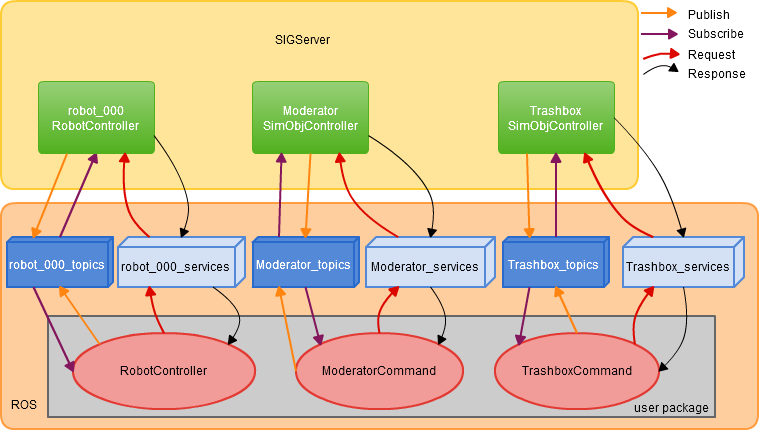
\includegraphics [width=150mm]{images/cleanUpNodes.png}}
\captionof{figure}{Controllers and nodes necessary to the Clean up task}\label{fig:cleanUpNodes}%      only if needed  
\end{minipage}

Three ``Controller'' are generated ``robot\_000'', ``Moderator'' and ``Trashbox'', with them the topics and services for each. By default, the name of the topics and services begins by the name of the ``Controller''.\\
Each script are inside three nodes: RobotCommand, ModeratorCommand and TrashboxCommand. It is the user part, he can program everything he wants to send messages to SIGServer. In this case, ``ModeratorCommand'' connects with the ``Referee'' service and send it messages, we can see the result on the left top corner in the video.\\
This is an easy example for the clean up task who can be find on the ``user'' package provided in the same repository as ``sig\_ros''.\\

Now, it is necessary to make this package capable of doing every movement for the robot, not only the clean up task. That is why just a mapping of every methods of SIGVerse to manipulate object and robot is necessary.\\
All topics and services availables are described in annex~\ref{annex:topics} and \ref{annex:services}.\\
A user manual is also available on the sig\_ros repository inside the doc folder of the sig\_ros package. This manual explains how to use the sig\_ros package and the example of the Clean up task.

\section{ROS package adapation}
\subsection{SLAM}
\subsubsection{Concept}\label{sec:slam_functionning}
The node SLAM take as entry two topics, /scan and /tf as we can see figure~\ref{fig:slam}. On the /scan topic, the information of the laser scan has to be published there. The type of the message is sensor\_msgs/LaserScan and the description can be found on \url{http://docs.ros.org/api/sensor_msgs/html/msg/LaserScan.html}. The ranges are the values of the distance between the robot and the next obtacle for each angle from angle\_min to angle\_max separated by angle\_increment on the positive way.\\
The range\_min and range\_max are respectively the min value and the max value possible for the range.\\
The intensity is not mandatory, it is the value for the obtacle transparence for the measurement.\\

The node subscribe to /tf too. /tf provide the tree of the robot from odometry to the laser place. That is why the minimum tree is /odom $\rightarrow$ /base\_link. Slam node also need /map $\rightarrow$ /odom but it provides it itself publishing to /tf.

The node publish to two topics and one service is available to get the map.\\

\noindent\begin{minipage}{\linewidth}% to keep image and caption on one page
\makebox[\linewidth]{%        to center the image
  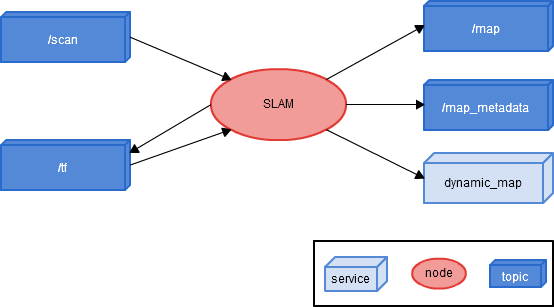
\includegraphics [width=150mm]{images/slam.png}}
\captionof{figure}{SLAM topics and services}\label{fig:slam}%      only if needed  
\end{minipage}

\subsubsection{Integration into SIGVerse}
As we saw section~\ref{sec:slam_functionning}, the topic scan and tf have to be published regularly. That is why the ``action'' will publish to the topics, because it is always called.\\
SIGVerse provide a laser scan for its robots, so the data only has to be modified to be on the /scan format.
For /tf, it is the same, but the tree has to be built depending on the robot. As the robot can be very different, I chose to build the easiest tree possible and assume that the laser scan is placed at the base\_link.\\

However, many problems occured due to a lack of documentation of the package. Indeed, the ros tutorial to use this package only explains the topics published and subscribed, services availables, parameters, and the type of the messages needed. But nothing about the meaning of the data needed. For example, the field ``range'' of the scan message has the description ``range data [m] (Note: values $<$ range\_min or $>$ range\_max should be discarded)'' but nothing says how the values are taken positive way, negative way, from 0 radian, from 90,...\\

There is two way to publish a message, publishing directly to a topic or send it by broadcast. /tf has to be sent by broadcast, but nothing informs the user.\\

Before the integration of this package to SIGVerse, I tried to use it with the turtlebot simulator, it worked, I could move the turtlebot robot and the map was built. The same has to be done with SIGVerse simulator but no documentation exists about how turtlebot simulator publish information to make the slam package worked.

\subsection{Inverse kinematics}
\subsubsection{Concept}
ROS provide a package for solving the inverse kinematics and an example is provided on the documentation with a robot called pr2. We can show pr2 with rviz\footnote{rviz is an 3D visualization tool for ROS} and launch a node from the tutorial to make move the robot in rviz using the inverse kinematics.\\
With this example, I was able to distinguish three parts of the work to realize, how the inverse kinematics package knows the description of pr2, how the information are sent to the ik package and how the result of the ik package is performed by rviz to make the robot moving. 

\subsubsection{Robot definition}
The ik package need two files, an urdf\footnote{Unified Robot Description Format} file to provide the description of the robot or an xacro file who generate the urdf file and a srdf\footnote{Semantic Robot Description Format} file which describe the semantic of the urdf file.\\

The SIGVerse robot is not the same as pr2, that is why the construction of an urdf file was necessary. Inside SIGVerse, the robot is described by an xml file which include non-standards x3d\footnote{A royalty-free ISO standard XML-based file format for representing 3D computer graphics} files. So, the transformation from x3d to urdf was not a good idea.\\
The best way was just modifying the urdf file of pr2 to look like the SIGVerse's robot.\\

The original urdf file had more than 4 000 lines, including ``transformation'' and gazebo tags. This two kind of tags are used by gazebo to make the robot moving easily, but inside SIGVerse, we do not need it, so the first step was to get rid of this tags.\\
Then, the urdf file is only made by ``link'' and ``joint'' tags. The structure of the file can be see as a tree starting by ``base\_link'' and putting a link between two joints. The origin of the child link of a joint make the length of its. We can see annex~\ref{annex:pr2Tree}, thanks to a tree, the original pr2 structure in the urdf file. \\
The second step was get rid of everything that the ik package does not need, some joints and links. At the same time, updating the srdf file removing the joints and links who are not necessary. The minimal structure of the robot can be see annex~\ref{annex:minStruct} \\
After that, it was just necessary to modify the size of the robot, height and arm's length related to the joints and links. For that I made a python script who modifies the length of the arms and the size of the robot of the file previously obtained.\\
Thanks to this script, the urdf file can be generated with the SIGVerse data. The robot can be changed just modifying the xml file for SIGVerse and if the robot has the same structure, the urdf file will be generated and the ik package will work as usual. The unique requirement is that the robot need the same structure.\\ 

Once the description file of the SIGVerse robot is built, it just need to fill the variable ``robot\_description'' of the ros launch file with the urdf file and the srdf file to make sure the ik package can access to the robot description.\\

\begin{figure}
\centering
\begin{subfigure}{.5\textwidth}
  \centering
  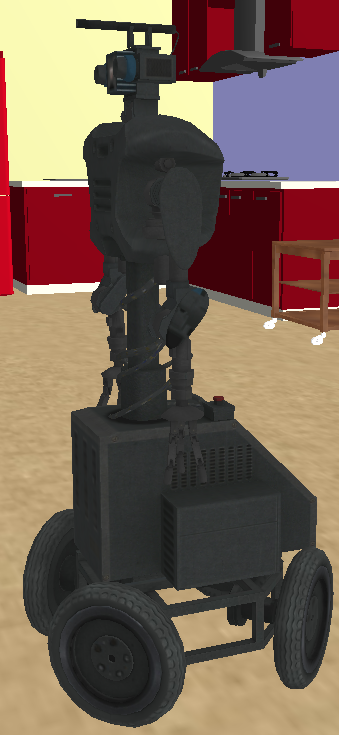
\includegraphics[width=50mm]{images/robot_000_sigverse.png}
  \caption{robot\_000 inside SIGVerse}
  \label{fig:robotSig}
\end{subfigure}%
\begin{subfigure}{.5\textwidth}
  \centering
  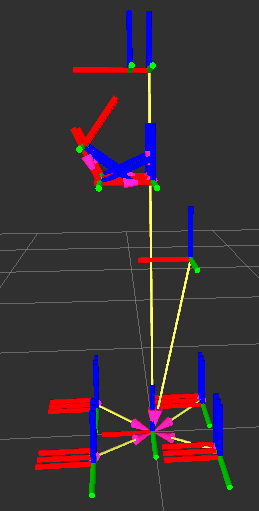
\includegraphics[width=55mm]{images/robot_000_rviz.png}
  \caption{robot\_000 described by urdf file}
  \label{fig:robotRviz}
\end{subfigure}
\caption{Visualisation of robot\_000}
\label{fig:robotVisu}
\end{figure}

We can see figure~\ref{fig:robotVisu}, the subfigure~\ref{fig:robotSig} shows the robot in the initial position inside SIGVerse and subfigure~\ref{fig:robotRviz} the same robot described by the urdf file viewed thanks to RViz. The robots have the same proportion but one difference is obvious, the position of the arms is not the same. A solution to this problem is explained section~\ref{subsubsec:integIKSIG}.\\
Between these two robots, another difference can be noticed, the orientation of the axis, indeed in SIGVerse y axis is vertical and x and z on the floor whereas in rviz, z is vertical.

\subsubsection{Result interpretation}
Once the ik package called, it answers a list of numbers corresponding to a list of joints names. The numbers are the angle in radian between the two links of a joint as we can see figure~\ref{fig:ikAngles}.
We can see the original position of the arm in red (it is the one showed in figure~\ref{fig:robotRviz}), the shoulder to the elbow measures 4 and the elbow to the wrist measures 3.21.\\
Then, if we ask for the position (0,1,0), the angle for the Elbow' is -0.813847 rad, that is why $\widehat{G,Elbow',Wrist'}$ = -46.63°.\\
For the shoulder, the angle with the original position and the new one will be -0.27157 rad for the position (0,1,0) and 0.23841 rad for the position (0,-1,0). The shoulder has 0 rad on its original position, indeed, we can see shoulderPan, shoulderLift and Elbow in the same line.

\noindent\begin{minipage}{\linewidth}% to keep image and caption on one page
\makebox[\linewidth]{%        to center the image
  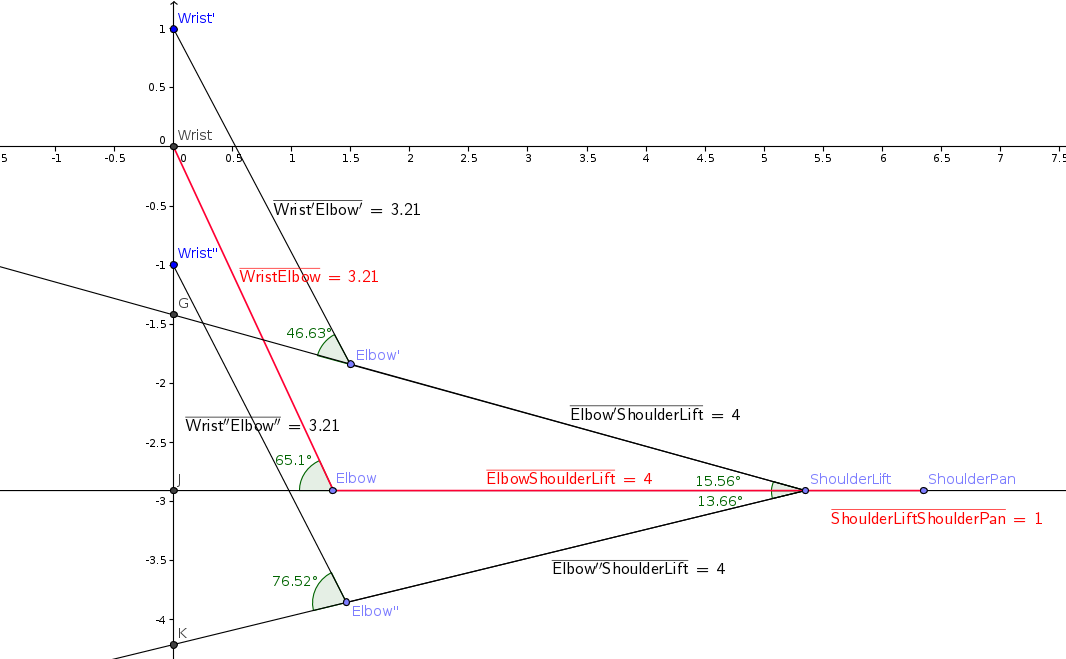
\includegraphics [width=150mm]{images/ggbAngles.png}}
\captionof{figure}{Angles between joints}\label{fig:ikAngles}%      only if needed  
\end{minipage}

\subsubsection{Integration into SIGVerse}\label{subsubsec:integIKSIG}
The ik package can figure out the position of every joint or not if the position of the end effector can not be reached. That is why I made a service, called ``\_ik'', available to use this package. The necessary data are simple, the position of the end effector hoped, the arm (left or right) whom the user wants to move and a last argument to provide the signification of the position.\\

We can see figure~\ref{fig:ikServ}, the concept for the use of the ik package is the same as a direct interaction with a robot (or object) inside SIGVerse. A service (ik) has to be called and the node RobotController will ask the ik package for the angles of each joints. After that, the RobotController interprets the result and make the arms of the SIGVerse robot moving.\\
The response by the service is necessary to notify the user node if the move has been possible (and so done) or not.

\noindent\begin{minipage}{\linewidth}% to keep image and caption on one page
\makebox[\linewidth]{%        to center the image
  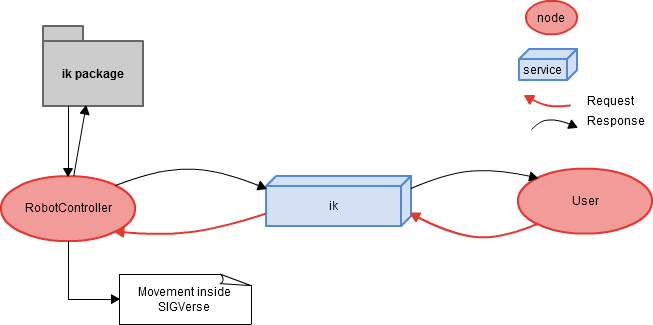
\includegraphics [width=150mm]{images/ik.png}}
\captionof{figure}{Architecture for the use of ik package}\label{fig:ikServ}%      only if needed  
\end{minipage}

The data position can be provided by three different form, absolute, relative or empty.\\
The empty form corresponds to the vector from the original position (0,0,0) and the new position.\\
The absolute position corresponds to the coordinates of SIGVerse where the user wants the arm to be.\\
The relative position corresponds to the vector from the current position to the new position.\\

The empty position does not need any treatment of the position given but the absolute and relative need to be modifyied. Indeed, the ik package need the data as the ``empty'' position, example figure~\ref{fig:ikAngles} the position (0,0,0) is the default position.\\
That is why, it was necessary to know the coordinate of the default position for calculate the vector from the default position to the wanted position. For that, I decided to apply matrix transformation to the arm hands position called ``Wrist''. See figure~\ref{fig:armCalculPoint} a visual of the problem.

\noindent\begin{minipage}{\linewidth}% to keep image and caption on one page
\makebox[\linewidth]{%        to center the image
  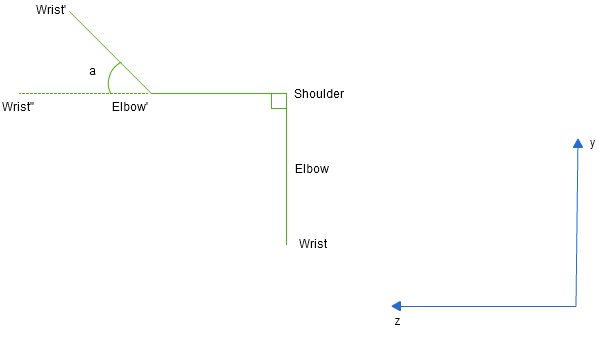
\includegraphics [width=130mm]{images/armCalculPoint.png}}
\captionof{figure}{Difference between the position of the arm in SIGVerse and RViz}\label{fig:armCalculPoint}%      only if needed  
\end{minipage}

In blue, we can see the axis of SIGVerse. The straight line Shoulder-Elbow-Wrist represents the initial position of the arm inside SIGVerse and the straight lines Shoulder-Elbow'-Wrist' the initial (default) position inside RViz.\\

The length of each part can be found thanks to SIGVerse and the angle ``a'' thanks to the ik package. Indeed, if we ask for the position (0,0,0) the angle ``a'' will be answered.\\
The computation of the points Elbow' and Wrist'' are easy, it is just the translation of the point Shoulder. For the point Wrist', I used matrix of transformation as follow:\\
Wrist' = T$_{-Elbow'}$ R$_{-a}$ T$_{Elbow'}$ Wrist'' with:\\

T$_{P}$ =
$\begin{pmatrix}
   1 & 0 & 0 & P_x \\
   0 & 1 & 0 & P_y \\
   0 & 0 & 1 & P_z \\
   0 & 0 & 0 & 1
\end{pmatrix}$ and 
R$_{\theta}$ = 
$\begin{pmatrix}
   1 & 0 & 0 & 0 \\
   0 & cos(\theta) & -sin(\theta) & 0 \\
   0 & sin(\theta) & cos(\theta) & 0 \\
   0 & 0 & 0 & 1
\end{pmatrix}$

This computation is made for both arms. This, allows the user to not having a symetric robot, he can decide of the length of each part independently.

\section{Internship progress}
\subsection{Discovery}
The first two weeks were dedicated to the installation of the environment: Operating System, Virtual Machine, SIGServer, SIGViewer. After that, I could see how SIGVerse works. 

Ones the environment installed, I was able to run examples of the wiki page \cite{SIGVerseWiki}. With this examples, I could see the function of the ``Controller'' and then understand how an agent can act, changing places, saying ``Hello'',... But also, how an agent communicates in both ways, sending and receiving messages.\\

After installing the environment and learning how to create an agents and make them move, I had to know what was ROS and how it is working. So, I installed all the environment and I did the tutorials of the wiki page \cite{ROSWiki}.\\
After that, I could run an example of SIGVerse running with ROS and then beginning to investigate how to design an interface between SIGVerse and ROS.

\subsection{Tools}
At the beginning, I was developping on a virtual machine Ubuntu 12.04, but few weeks later SIGVerse was officially available on Ubuntu 14.04, the stablest version where SIGVerse works well. Because of many troubles on Ubuntu 12.04, I decided to upgrade to Ubuntu 14.04.\\
No IDE\footnote{Integrated Development Environment} is used, only a text editor gedit and a terminal for compilation. ROS and SIGVerse are open source so, I decided to use GitHub.\\
Because of the reinstallation of the virtual machine, a behaviour was not expected, un keyboard problem, so I decided to change my text editor to vim\footnote{Visual Interface IMproved}.\\ 
I am using Windows 8.1 for the compatibility with the kinect which I could need during the project.\\

I used Geogebra software to verify my theories about the angles answered by the inverse kinematics package.\\

I used Cacoo on line to make every schema of this report.\\

I make unit tests with ROS to be sure of the good functioning.

\subsection{Organisation}
The choice of my subject was very open, my supervisor showed me the simulator SIGVerse and the first step after the installation was finding a subject. Because of the short time due to the DoW\footnote{Description of Work} deadline, I chose to work on this project.\\
After the three first months, the main part was done, that means the Clean up task demo and the development of topics and services necessary to have a full access to SIGVerse functionnalities from ROS.\\
After that, I started to add functionnalities to my package. This new functionnalities are an adaptation of the use of a ROS package to SIGVerse. I included the SLAM and inverse kinematics package.\\

Once a week, all laboratory's members attends a meeting where each members exposes what he planned to do last week, what he actually did and what he will do the next week. I make my own objectives every week for achieving the main goal.\\
My supervisor answers to my questions and gives me indications during the meeting.

\subsection{Troubles}
\subsubsection{Development}
First of all, due to my lack of knowledge about ROS, it was very difficult to gain a full view of the project at the beginning. That is why, I had to spend some days to learn from the ROS tutorials and to practice with this framework.\\
When I started implementing the ``Controller'', I had a problem of inheritance. Indeed, I had to inherit the robot ``Controller'' from the object ``Controller'' and keep this two ``Controller'' usable for an agent. This inheritance was not easy because of ROS.\\
I found SIGVerse bug using a function ``getSimulationTime()'' and others functions. I spent a lot of time diagnosing this bug because I though it came from my code but finally it was a SIGVerse error. So, I made a bug report, sometimes it is just the function who does not answer the good thing, sometimes if we put a wrong arguments, the all simulator can stop.

\subsubsection{Documentation}
The documentation of SIGVerse is in japanese, so it is quiet difficult to understand what every method does, so I did a lot of tests to figure it out. Fortunately, Google translate can be a good help.\\

For the adaptation of the package SLAM and inverse kinematics, we can find a lot of tutorials to use this packages but none of them explains how they works.\\
For example, we can find turtlebot and a simulator of its. Using the simulator Rviz, we can make the SLAM package works, the data send by turtlebot make possible the computation of the map. If I register the messages sent by turtlebot and then I send it from SIGVerse, it works, but if I make my own messages, it is not working. But no information can be found about this messages, just the structure but not the containt. So, I asked for the help of the community, posting a message on the forum.\\

For the inverse kinematics package, it is the same problem, there was no information neither the interpretation of the result nor how to set the description of the robot. I figured it out thanks to the examples, trying to understand how it was working.

\subsubsection{Conception}
The objective of this interface is increasing the number of SIGVerse users by adding ROS users. So, the use of my package has to be instinctive, so the choice of the topics and services has to be relevant.\\
I made the choice to add an argument to each topics or services called ``name'', this argument is the same for all of them, that means the object or robot to whom it is applyied.\\

For the inverse kinematics, I chose to make available three types of position: relative, absolute and respect to the ``default'' position.\\
The computation of the default position inside SIGVerse was not easy because of two centimeters less than I had to find. The source of this two centimeters issue was no obvious, it can be because of the robot description, the computation itself or SIGVerse. But this issue is quit important because if the user ask for example for the position (116.64, 85, 42), the inverse kinematics package will answer it not find a solution because the computation of the default position is (116.64, 90, 40) and not (116.64, 90, 42), so my package will ask for the vector (0, -5, 2) instead of (0, -5, 0).

\subsection{Schedule}
\subsubsection{What I planned}
In the DoW report, I planned to achieve the job L2 before the mid-term report deadline. That means make SIGVerse works with ROS by a simple way like one ``Controller'' with one node and generate a ``Controller'' for each agent on the simulator.\\

After that, I planned to design and develop the topics and services that are necessary to control the agents. I also planned to make an interface between the real human and the simulator. For example, making work the kinect. We can see annex~\ref{GanttChart} the schedule of the DoW.

\subsubsection{What I actually did}
Finally, the first part (before de mid-term report about making work a simple ``Controller'' with one node) was easier than I though and I could start the next job. So, I started implementing some topics and services for the clean up task before the mid-term report.\\
Only the methods for the clean up task have been done and some others. You can see at \url{https://www.youtube.com/watch?v=PL4MCjire2M&feature=youtu.be} a demonstration of the clean up task. The actions of the robot are sent by ROS.\\

After that, I finished to develop the others topics and services for an all control of the robot. Then, I dealt with the referee during one month.\\
At this point, a demonstration was possible at a weekly meeting, the video of it is available here \url{https://www.youtube.com/watch?v=Fc38tqwr0F0&feature=youtu.be}. We can see the robot going for the trash and the referee at the left top corner counting the points.

Then, 3 months left so I decided to make more tests and I found bug on my package and on SIGVerse. After that, I made an adaptation of two ROS package who can provide more functionnalities to SIGVerse.\\
We can see figure~\ref{GanttChart:final} the schedule who actually occured.

\subsubsection{Reason of the changement}
The first changement has been made because it was easier than I though, but then, the second part has been changed because it was more interesting to add functionnalities to SIGVerse than adding the kinect.\\
Indeed, SLAM and inverse kinematics are two useful tools for every user, not only for those who use the kinect.

\subsubsection{To continue}

\begin{landscape}
%\subsection{Schedule}\label{sec:schedule}
%\thispagestyle{empty}
%\thispagestyle{plain}
\setlength{\topmargin}{25pt}
\titlespacing{\subsection}{0cm}{0cm}{0cm}


\noindent\begin{ganttchart}[
hgrid,
vgrid,% = {*6{white}, *1{black}},% *{10}{blue, dashed}},
x unit=0.3cm,
%title/.style={fill=teal, draw=none},
%title label font=
%\color
%{white}
%\bfseries,
inline,
time slot format=isodate,
]{2015-03-16}{2015-06-07}
\gantttitlecalendar{year, month=name, week}{4} \\
\ganttbar{Planification}{2015-03-16}{2015-04-12}
\ganttbar{Project monitoring}{2015-04-13}{2015-06-07}\\

\ganttbar{DoW Report}{2015-04-03}{2015-04-12}
\ganttbar{Environment installation}{2015-03-16}{2015-03-28}
\ganttbar{Tutorials}{2015-03-29}{2015-04-02}
\ganttbar{L2:T1}{2015-04-13}{2015-04-19}
\ganttmilestone{DoW}{2015-04-12}
\ganttbar{L2:T2}{2015-04-20}{2015-05-03}
\ganttbar{L2:T3}{2015-05-04}{2015-05-10}
\ganttbar{L3:T1}{2015-05-18}{2015-06-07}\\

\ganttbar{Technical documentation}{2015-04-13}{2015-05-10}
\ganttbar{Technical documentation}{2015-05-18}{2015-06-07}\\

\ganttbar{Mid-term Report}{2015-05-04}{2015-05-17}
\ganttmilestone{Mid-term report}{2015-05-17}

\end{ganttchart}

\noindent\begin{ganttchart}[
hgrid,
vgrid,
x unit=0.3cm,
inline,
time slot format=isodate,
]{2015-06-08}{2015-08-30}
\gantttitlecalendar{month=name, week = 13} \\
\ganttbar{Project monitoring}{2015-06-08}{2015-08-30}\\
\ganttbar{L3:T2}{2015-06-08}{2015-06-28}
\ganttbar{L4:T1}{2015-06-29}{2015-07-12}
\ganttbar{L4:T2}{2015-07-13}{2015-08-02}
\ganttbar{Final Report}{2015-08-10}{2015-08-30}\ganttmilestone{Final Report}{2015-08-30}\\
\ganttbar{Technical documentation}{2015-06-08}{2015-08-02}
\ganttbar{User documentation}{2015-08-03}{2015-08-16}
\end{ganttchart}
\captionof{figure}{Schedule of the internship}\label{GanttChart:final}
\end{landscape}

